\chapter{Forces, quarks et premiers multiplets de hadrons}

\section{Particules, champs et troisième élément manquant}

Les ondes sont des configurations de champs ; dans la discussion qui nous occupe, ces deux descriptions sont donc étroitement liées. La mécanique quantique nous dit que l’énergie d’une telle onde se présente sous forme d’unités discrètes et indivisibles. Ce sont ses quanta, et les quanta d’un champ sont ce que nous appelons ses particules. Avec cette relation en tête, nous avons déjà étudié les équations d’onde, les principes d’action et les grandes propriétés portées par les particules : énergie, quantité de mouvement, spin et distinction boson--fermion. Les fermions ne peuvent pas occuper le même état ; les bosons, eux, peuvent s’y rassembler et se condenser.

Un lagrangien quantique consigne également les interactions. Les produits de champs représentent des sommets auxquels des particules entrent et d’où elles sortent. Un terme comportant quatre puissances d’un champ, par exemple, représente un sommet d’interaction à quatre jambes. C’est ainsi que le principe d’action fournit un inventaire concis des processus particulaires possibles.

La tâche suivante consiste à nommer les particules---pas tout à fait une par une, mais par familles---et à donner à chacune une personnalité : ses propriétés, ses interactions et sa place dans la physique ordinaire. Avant d’en dresser la liste, il manque toutefois encore un côté au triangle conceptuel :
\begin{itemize}
\item les particules,
\item les champs dont ces particules sont les quanta,
\item les forces associées aux processus d’échange mettant en jeu ces mêmes quanta.
\end{itemize}

Le terme \emph{élémentaire} doit rester provisoire. Toute définition plausible d’une particule élémentaire, par opposition à une particule composite, finit par se heurter à un cas délicat, et nous reviendrons sur ce problème. Pour l’instant, supposons qu’il existe des champs fondamentaux et appelons particules élémentaires leurs quanta. Si un champ électrique engendre des forces électriques et un champ gravitationnel des forces gravitationnelles, alors le champ de l’électron doit lui aussi participer à des forces. Le triangle ne peut se refermer que si la force possède une description en termes de particules autant qu’en termes de champs.

Nous allons donc dériver deux fois la logique de la force. Nous commencerons par l’énergie classique des champs, puis nous demanderons comment la même interaction apparaît lorsque l’on décompose un champ en quanta. Ce n’est qu’une fois cette passerelle établie que nous commencerons le catalogue des particules.

\section{La force à partir de l’énergie des champs en électrodynamique classique}

Plaçons deux charges dans l’espace. Pour déterminer la force qu’elles exercent, on peut invoquer la loi en inverse du carré de la distance. Une approche plus éclairante consiste à demander ce que les charges font à l’espace : elles créent des champs électriques, et ces champs stockent de l’énergie.

Il est utile de séparer chaque charge de la forme spatiale de son champ,
\begin{equation}
\mathbf E_i=q_i\widehat{\mathbf E}_i,
\end{equation}
bien que rien ne dépende du maintien de la notation avec chapeau. En présence des deux charges, la linéarité donne
\begin{equation}
\mathbf{E}=\mathbf{E}_1+\mathbf{E}_2.
\end{equation}
À un choix d’unités près, l’énergie électrostatique du champ s’écrit
\begin{equation}
U_{\text{field}}\propto\int d^3x\,\mathbf{E}^2.
\end{equation}
En substituant la somme des deux champs, on obtient
\begin{align}
U_{\text{field}}
&\propto\int d^3x\,(\mathbf{E}_1+\mathbf{E}_2)^2 \\
&\propto\int d^3x\,\bigl(\mathbf{E}_1^2+\mathbf{E}_2^2
  +2\mathbf{E}_1\!\cdot\!\mathbf{E}_2\bigr).
\end{align}

Les deux premiers termes sont des énergies propres. La translation de l’une ou l’autre charge déplace son champ avec elle et ne modifie pas l’intégrale correspondante. Cette énergie contribue, par l’intermédiaire de \(E=mc^2\), à la masse mesurée de la particule chargée isolée. La manière dont cette énergie propre est prise en compte dans la masse mesurée relève du sujet ultérieur de la renormalisation. Aucune de ces énergies, indépendantes de la position, ne contribue à la force entre les deux particules.

Le terme croisé est différent. Il n’appartient à aucune particule prise séparément et n’existe qu’en présence des deux champs. Si les charges sont très éloignées l’une de l’autre, les régions où leurs champs sont appréciables se recouvrent à peine. À mesure que les charges se rapprochent, le recouvrement change. L’énergie d’interaction, qui dépend de la configuration, est donc proportionnelle à
\begin{equation}
U_{\text{int}}(r)\propto q_1q_2\int d^3x\,
\widehat{\mathbf E}_1\!\cdot\!\widehat{\mathbf E}_2.
\end{equation}
Pour deux charges ponctuelles séparées par \(r\), le calcul de l’intégrale donne la dépendance bien connue
\begin{equation}
U_{\text{int}}(r)\propto\frac{q_1q_2}{r}.
\end{equation}
La force radiale est l’opposé de son gradient,
\begin{equation}
\mathbf F_{12}=-\boldsymbol\nabla_{\mathbf r}U_{\text{int}},
\qquad
|\mathbf F_{12}|\propto\frac{|q_1q_2|}{r^2}.
\end{equation}
\editorialnote{L’argument oral identifie le terme croisé à la force de Coulomb en inverse du carré de la distance, sans s’arrêter au potentiel. Le terme intermédiaire usuel \(U_{\mathrm{int}}\propto1/r\) est écrit explicitement ici afin que son gradient donne la force \(1/r^2\) indiquée.}

La loi de force est devenue la dérivée de la partie de l’énergie du champ qui dépend de la position relative. À grande distance, les deux objets sont effectivement indépendants. Rapprochons-les : le champ entre eux se réorganise ; la variation d’énergie qui en résulte constitue l’interaction.

Mais si un champ peut être décomposé en quanta, l’histoire ne peut pas s’arrêter là. Il faut aussi rendre compte de la même force en termes de particules.

\section{Échange moléculaire : deux protons et un électron}

Avant de revenir à l’électrodynamique, considérons un système où l’échange est plus facile à se représenter : deux protons et un électron. L’échange n’est qu’une des diverses origines des forces moléculaires, mais cet exemple rend visible le lien entre échange, énergie et force. Il ne se substitue pas à l’électrodynamique quantique.

Si un proton est présent et que l’autre se trouve à l’infini, l’électron peut occuper l’état fondamental hydrogénoïde centré sur le premier proton. Sa fonction d’onde est localisée près de ce centre de force.

\begin{figure}[h]
\centering
\includegraphics[width=0.72\textwidth]{lecture_01_figure_02.png}

\medskip

\begin{tikzpicture}[scale=0.95]
\draw (-0.2,0) -- (6.4,0);
\fill (1.3,0) circle (2pt);
\draw[smooth] plot coordinates {(0.1,0.15) (0.8,1.15) (1.5,1.75) (2.2,1.1) (3.0,0.35) (3.8,0.12)};
\node at (1.3,-0.35) {$p$};
\node at (2.7,1.55) {$\psi_1(x)$};
\end{tikzpicture}
\caption{Fonction d’onde de l’état fondamental hydrogénoïde localisée près d’un proton.}
\lectureframe{00:14:32}
\end{figure}
\editorialnote{Dans le nouveau dessin, l’étiquette \(\psi_1(x)\) désigne le profil localisé décrit à 00:14:30--00:14:32 ; elle ne provient pas d’une étiquette lisible au tableau.}

Plaçons maintenant un second proton à une distance grande mais finie. Par symétrie, il existe un second état localisé, d’énergie identique pour un seul centre, cette fois centré sur le proton de droite.

\begin{figure}[h]
\centering
\includegraphics[width=0.78\textwidth]{lecture_01_figure_03.png}

\medskip

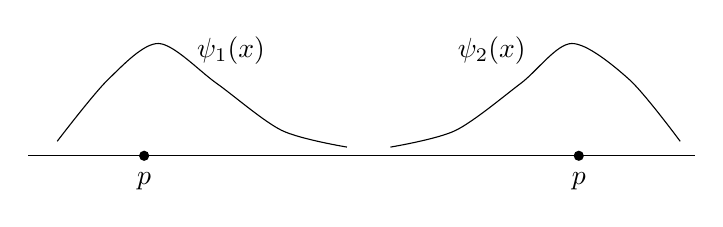
\begin{tikzpicture}[scale=0.92]
\draw (-0.2,0) -- (9.0,0);
\fill (1.4,0) circle (2pt);
\fill (7.4,0) circle (2pt);
\draw[smooth] plot coordinates {(0.2,0.2) (0.9,1.05) (1.6,1.55) (2.4,1.0) (3.3,0.35) (4.2,0.12)};
\draw[smooth] plot coordinates {(4.8,0.12) (5.7,0.35) (6.6,1.0) (7.3,1.55) (8.1,1.05) (8.8,0.2)};
\node at (1.4,-0.35) {$p$};
\node at (7.4,-0.35) {$p$};
\node at (2.6,1.45) {$\psi_1(x)$};
\node at (6.2,1.45) {$\psi_2(x)$};
\end{tikzpicture}
\caption{Les deux profils localisés utilisés pour former la superposition d’équilibre lorsque le tunnel est autorisé.}
\lectureframe{00:17:54}
\end{figure}
\editorialnote{Les étiquettes \(\psi_1(x)\) et \(\psi_2(x)\) désignent les deux profils évoqués à 00:17:41--00:17:56 ; il s’agit de repères schématiques ajoutés pour améliorer la lisibilité.}

À séparation infinie, les deux états sont dégénérés : localiser l’électron à gauche ou à droite coûte la même énergie. À séparation finie, un nouveau processus devient possible. L’électron peut traverser par effet tunnel la région classiquement interdite et passer d’un centre à l’autre. Chercher à suivre une trajectoire à travers la barrière perturberait l’état ; le ``saut'' décrit une évolution quantique, et non le film d’un parcours classique.

À l’équilibre, l’électron a la même probabilité de se trouver près de chacun des protons. La normalisation fournit donc le facteur \(1/\sqrt2\), et l’état d’équilibre de plus basse énergie est approximativement
\begin{equation}
\psi_+(x)\approx \frac{\psi_1(x)+\psi_2(x)}{\sqrt2}.
\end{equation}

Le signe d’approximation est important. La véritable fonction d’onde à deux centres n’est pas exactement la somme de deux orbitales hydrogénoïdes non perturbées ; elle s’ajuste dans la région de recouvrement. Ce qui importe ici, c’est que l’état symétrique d’équilibre a une énergie inférieure à celle du centre isolé. En termes hamiltoniens, les configurations gauche et droite sont couplées par un élément de matrice hors diagonale. Permettre à l’électron d’occuper leur superposition cohérente a abaissé l’énergie.

\section{De l’abaissement de l’énergie à une force effective}

À grande distance entre les protons, la contribution \(E_e(r)\) induite par l’électron tend vers sa valeur pour des atomes séparés. À plus faible distance, le tunnel et la superposition l’abaissent. Le potentiel complet des deux protons--un électron doit aussi inclure leur répulsion directe,
\begin{equation}
V_{\mathrm{tot}}(r)=V_{pp}(r)+E_e(r).
\end{equation}

Cela relie l’exemple moléculaire à l’argument fondé sur l’énergie des champs. Les schémas de fonctions d’onde et la courbe qualitative de \(E_e(r)\) représentent deux aspects du même calcul ; l’équilibre est déterminé par la somme \(V_{\mathrm{tot}}(r)\).

\begin{figure}[h]
\centering
\includegraphics[width=0.78\textwidth]{lecture_01_figure_04.png}

\medskip

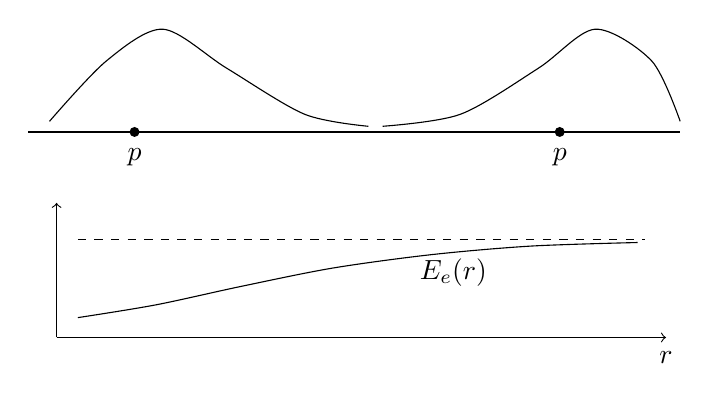
\begin{tikzpicture}[scale=0.9]
\draw (-0.2,3.0) -- (9.0,3.0);
\fill (1.3,3.0) circle (2pt);
\fill (7.3,3.0) circle (2pt);
\draw[smooth] plot coordinates {(0.1,3.15) (0.9,4.0) (1.7,4.45) (2.6,3.9) (3.7,3.25) (4.6,3.08)};
\draw[smooth] plot coordinates {(4.8,3.08) (5.9,3.25) (7.0,3.9) (7.8,4.45) (8.6,4.0) (9.0,3.15)};
\node at (1.3,2.65) {$p$};
\node at (7.3,2.65) {$p$};

\draw[->] (0.2,0.1) -- (0.2,2.0);
\draw[->] (0.2,0.1) -- (8.8,0.1);
\draw[dashed] (0.5,1.48) -- (8.5,1.48);
\draw[smooth] plot coordinates {(0.5,0.38) (1.6,0.56) (2.8,0.82) (4.1,1.08) (5.5,1.27) (6.9,1.39) (8.4,1.44)};
\node at (5.8,1.02) {$E_e(r)$};
\node at (8.8,-0.18) {$r$};
\end{tikzpicture}
\caption{Recouvrement des fonctions d’onde en haut et énergie induite par l’électron en bas. Cette énergie tend vers l’asymptote des atomes séparés lorsque \(r\) augmente ; le potentiel total des protons doit aussi inclure leur répulsion coulombienne.}
\lectureframe{00:20:28}
\end{figure}
\editorialnote{Les étiquettes \(E_e(r)\) et \(r\) désignent la courbe d’énergie et la séparation évoquées à 00:19:12--00:20:38 ; l’image du tableau conservée ne permet pas de lire les étiquettes des axes.}

Les deux forces correspondantes découlent des gradients de l’énergie,
\begin{equation}
F_{e}(r)=-\frac{dE_e}{dr},
\qquad
F_{\mathrm{tot}}(r)=-\frac{dV_{\mathrm{tot}}}{dr}.
\end{equation}
Le système est donc poussé vers une énergie totale plus basse. Là où \(E_e(r)\) diminue à mesure que les protons se rapprochent, l’échange apporte une contribution attractive ; l’existence ou non d’une distance d’équilibre dépend de la compétition avec \(V_{pp}(r)\). C’est le mécanisme élémentaire à l’origine d’une liaison covalente : l’électron est partagé parce que l’état partagé est énergétiquement favorable.

Dans le calcul classique, le recouvrement des champs électriques modifie l’énergie. Ici, deux centres de force permettent d’abaisser l’énergie d’un état quantique. Dans les deux cas, une force apparaît parce que l’énergie d’équilibre dépend de la configuration.

On peut résumer le langage de l’échange par un schéma de lignes d’univers. Il ne faut pas le lire comme une trajectoire observée ; il représente les amplitudes correspondant aux associations possibles de l’électron avec l’un ou l’autre proton.

\begin{figure}[h]
\centering
\begin{tikzpicture}[scale=1.0]
\draw (0,0) -- (0,4.4);
\draw (4.8,0) -- (4.8,4.4);
\draw (0,0.9) .. controls (1.6,1.7) and (3.2,1.7) .. (4.8,2.5);
\draw (4.8,2.9) .. controls (3.2,2.1) and (1.6,2.1) .. (0,3.9);
\node at (0,-0.35) {$p$};
\node at (4.8,-0.35) {$p$};
\node at (2.35,1.55) {$e^-$};
\node at (2.35,2.55) {$e^-$};
\end{tikzpicture}
\caption{Échange électronique entre deux lignes d’univers de protons, schématisé par des amplitudes quantiques plutôt que par une trajectoire suivie.}
\end{figure}

\begin{classroomqa}
\audiencequestion{L’attraction s’explique-t-elle simplement par l’écrantage de l’électron, qui réduirait la charge du proton ?\lecturetimestamp{00:23:26}}
\lecturerresponse{Non. La réduction de charge n’est pas une bonne façon de se représenter cet effet. L’essentiel est que la combinaison des deux fonctions d’onde localisées produit un état dont l’énergie est légèrement inférieure à celle de chacun des états localisés pris séparément.}
\end{classroomqa}

\begin{classroomqa}
\audiencequestion{Est-ce ce que Feynman voulait dire en disant que ``la lumière aime la lumière'' ?\lecturetimestamp{00:23:51}}
\lecturerresponse{Non. Cette expression concerne très probablement la statistique de Bose : les photons favorisent les états communs, tandis que les électrons obéissent au principe d’exclusion. L’effet moléculaire dont il est question ici est le tunnel entre deux centres.}
\end{classroomqa}

Les deux protons continuent de se repousser électrostatiquement. L’échange est de plus courte portée que l’interaction coulombienne ; il faut donc considérer le potentiel total, et non l’une ou l’autre contribution isolément. Pourtant, à certaines distances, l’ion moléculaire \(\mathrm H_2^+\) est lié ; dans un système neutre à deux électrons, la répulsion électrique à longue portée est absente et la liaison covalente est encore plus familière.

\begin{classroomqa}
\audiencequestion{Le fait de placer l’électron entre les protons réduit-il surtout leur répulsion électrostatique ?\lecturetimestamp{00:24:33}}
\lecturerresponse{Il réduit un peu la répulsion, mais ce n’est pas l’effet principal. La force due à l’échange électronique a une portée plus courte que la répulsion coulombienne. Elle apparaît le plus clairement dans un système neutre à deux électrons, où la force électrostatique à longue portée entre les atomes est absente, mais où le tunnel produit toujours une attraction.}
\end{classroomqa}

\begin{classroomqa}
\audiencequestion{L’ion moléculaire chargé positivement \(\mathrm H_2^+\), qui ne possède qu’un électron, est-il réellement lié ?\lecturetimestamp{00:26:06}}
\lecturerresponse{Oui. À suffisamment faible distance, l’attraction due à l’échange est assez forte pour surmonter la répulsion coulombienne proton--proton.}
\end{classroomqa}

\begin{classroomqa}
\audiencequestion{La configuration à deux centres crée-t-elle une troisième force ?\lecturetimestamp{00:26:24}}
\lecturerresponse{Aucune nouvelle force fondamentale n’est introduite. L’équation de Schr\"odinger dans le potentiel combiné des deux protons a une énergie d’équilibre différente de celle du problème à un centre ; la dérivée de cette énergie modifiée est la force effective.}
\end{classroomqa}

\begin{classroomqa}
\audiencequestion{L’abaissement de l’énergie est-il un exemple d’intrication quantique ?\lecturetimestamp{00:27:06}}
\lecturerresponse{Pas au sens habituel d’un système à deux particules : un seul électron suffit. La caractéristique mathématique pertinente est un élément de matrice hamiltonien hors diagonale qui couple les états gauche et droite.}
\end{classroomqa}

\begin{classroomqa}
\audiencequestion{Que devient l’échange à haute température ?\lecturetimestamp{00:27:37}}
\lecturerresponse{À température extrême, l’électron est ionisé et ne fait plus du tout partie de la molécule. À une énergie d’excitation plus basse, il peut occuper une orbitale plus grande, ce qui modifie le recouvrement et donc la force. Il s’agit d’une correction dépendant de l’état, et non d’un nouveau mécanisme général.}
\end{classroomqa}

\section{L’échange de photons et les premières entrées du tableau}

Peut-on décrire aussi la force de Coulomb en termes d’échange ? Une particule chargée interagit avec le champ électromagnétique, dont les quanta sont les photons. Classiquement, nous déterminons le champ électrique autour de la charge. En théorie quantique des champs, nous décomposons cette interaction en émission et absorption de photons.

Une particule chargée physique n’est pas simplement une charge nue. Son état est une superposition quantique qui comporte une composante d’électron nu, un électron avec un photon, un électron avec deux photons, et ainsi de suite. En notation volontairement schématique,
\begin{equation}
\begin{aligned}
\ket{e_{\mathrm{phys}}}
={}&a_0\ket e
+a_1\ket{e+\text{one photon}}
\\
&+a_2\ket{e+\text{two photons}}+\cdots .
\end{aligned}
\end{equation}
Cette notation indique uniquement la hiérarchie des composantes selon le nombre de photons ; elle ne précise pas leurs impulsions et ne prétend pas construire intégralement un état chargé en interaction.
Les photons qui l’entourent sont émis puis réabsorbés, plutôt que de s’échapper sous forme de rayonnement libre. Leurs effets sont mesurables, bien qu’on ne les détecte pas de la même façon que des photons se propageant librement. Plaçons une seconde charge à proximité : un photon émis par l’une peut être absorbé par l’autre. L’énergie des deux états habillés n’est alors plus la simple somme de deux énergies isolées.

L’analogie utilisée en cours met en scène deux jongleurs, qui manipulent chacun un jeu de balles. Lorsqu’ils sont éloignés, chacun jongle de son côté. Rapprochons-les suffisamment : l’un peut rattraper une balle lancée par l’autre. Dans le langage des diagrammes de Feynman, cet objet partagé est le photon échangé. L’analogie ne décrit pas une trajectoire microscopique, mais montre pourquoi la proximité permet un nouveau processus.

Nous disposons maintenant de deux descriptions qui vont au-delà de la simple mémorisation de la loi de Coulomb. La théorie classique des champs additionne les champs puis élève le résultat au carré. La théorie quantique des champs somme les amplitudes correspondant à des échanges de quanta. En ce sens, particules, champs et forces forment une correspondance un pour un. Les électrons médiatisent l’échange moléculaire, les photons l’échange électromagnétique, et toute particule susceptible d’être échangée peut contribuer à une force dans un contexte approprié. Ainsi, l’énoncé bien connu selon lequel la nature possède quatre interactions fondamentales relève d’une classification plus générale ; dans le langage de l’échange, chaque espèce susceptible d’être échangée peut engendrer sa propre contribution à une force effective.

Il est enfin temps de nommer les particules, d’énumérer leurs propriétés et d’indiquer à quels processus elles peuvent participer. Écrire d’un seul coup tout le Modèle standard ne produirait qu’un long exercice de mémorisation ; nous répartirons donc les particules en petits groupes dont les membres sont liés simplement et apprendrons ce que chacun peut faire.

Le catalogue complet est difficile à manier parce que nous ne comprenons pas pourquoi ce sont précisément ces particules qui existent, et non d’autres particules imaginables. La cohérence mathématique impose certaines relations : une fois que plusieurs membres d’un motif existent, un autre peut être nécessaire pour le compléter. Ces relations réduisent le nombre de faits indépendants, mais seulement dans une mesure modeste. De nombreux types de particules et de nombreux paramètres restent inexpliqués. Comprendre cette structure encore inachevée est nécessaire pour comprendre ce que les expériences ultérieures cherchent à découvrir.

\begin{figure}[h]
\centering
\includegraphics[width=0.7\textwidth]{lecture_01_figure_05.png}
\caption{La première entrée du tableau des particules identifie le photon par \(\gamma\) et son champ par le potentiel vecteur \(A\).}
\lectureframe{00:39:11}
\end{figure}

La première identification champ--quantum est
\begin{equation}
\gamma \leftrightarrow A.
\end{equation}
Ici, \(A\) est le potentiel vecteur électromagnétique. Le photon est un boson de spin un, de charge électrique nulle, de nombre baryonique nul et de masse au repos nulle. Le champ de l’électron est traditionnellement noté \(\psi_e\) ; ses parties de création et d’annihilation agissent sur les états d’électron et de positron.

Notre tableau consigne le nom, le symbole de la particule, le champ, le type boson ou fermion, la charge électrique \(Q\), le nombre baryonique \(B\) et la masse :

\begin{table}[h]
\centering
\resizebox{\linewidth}{!}{%
\begin{tabular}{lllllll}
Nom & Symbole & Champ & Type & \(Q\) & \(B\) & Masse \\
Photon & \(\gamma\) & \(A\) & boson & \(0\) & \(0\) & \(0\) \\
Électron & \(e^-\) & \(\psi_e\) & fermion & \(-1\) & \(0\) & \(0.51\,\mathrm{MeV}\) \\
Positron & \(e^+\) & \(\psi_e\) & fermion & \(+1\) & \(0\) & \(0.51\,\mathrm{MeV}\)
\end{tabular}
}%
\caption{Le photon et les entrées de l’électron--positron qui ouvrent le catalogue des particules.}
\end{table}

La relation entre l’électron et le positron est réciproque : chacun est l’antiparticule de l’autre. Appeler l’état chargé négativement ``la particule'' relève d’une convention. Nous mesurons la charge électrique en unités de la valeur absolue de la charge de l’électron, de sorte que
\begin{equation}
Q(e^-)=-1,\qquad Q(e^+)=+1.
\end{equation}
On mesure la masse en unités d’énergie en utilisant \(E=mc^2\). Un électronvolt est l’énergie acquise par une charge \(e\) soumise à une différence de potentiel d’un volt,
\begin{equation}
1\,\mathrm{eV}=e\,(1\,\mathrm V).
\end{equation}
Cette unité vient naturellement de la physique atomique : comme échelle atomique approximative, l’ionisation de l’hydrogène coûte environ \(13.5\,\mathrm{eV}\). Les masses des particules nécessitent des millions ou des milliards d’électronvolts. La masse de l’électron est
\begin{equation}
m_e c^2 \approx 0.511\,\mathrm{MeV}.
\end{equation}

\begin{classroomqa}
\audiencequestion{La masse de l’électron devrait-elle être exactement égale à un demi-MeV ?\lecturetimestamp{00:44:02}}
\lecturerresponse{Non. La valeur arrondie pratique \(0.51\,\mathrm{MeV}\) n’est fixée à un demi exact par aucun principe ; c’est un paramètre mesuré.}
\end{classroomqa}

Le processus élémentaire de l’électrodynamique quantique comporte une ligne de fermion chargé qui entre, une qui sort et une ligne de photon attachée au sommet. Réarranger les jambes ou les croiser permet au même sommet de décrire l’émission, l’absorption d’un photon ou un processus faisant intervenir un positron. Dans la notation schématique non covariante employée ici, l’interaction comporte
\begin{equation}
\mathcal{L}_{\mathrm{int}}\sim e\,\psi_e^\dagger \psi_e A.
\end{equation}
Le développement des champs en opérateurs de création et d’annihilation produit des termes qui retirent un électron incident, créent un électron sortant et créent ou annihilent un photon. Le couplage \(e\) fournit un facteur au sommet. Ainsi, lors de l’émission d’un photon par un électron diffusé ou accéléré,
\begin{equation}
\mathcal{A}_{\mathrm{vertex}}\propto e,
\qquad
P_{\mathrm{emission}}\propto e^2.
\end{equation}
L’impact d’un électron sur la cible d’un tube à rayons X est un exemple pratique où cette probabilité d’émission de photons intervient. Des combinaisons répétées du même sommet engendrent les processus de l’électrodynamique quantique, notamment le décalage d’énergie interprété comme la force entre charges.

Un sommet schématique est donc utile.

\begin{figure}[h]
\centering
\begin{tikzpicture}[scale=1.0]
\fill (0,0) circle (1.5pt);
\draw (-1.6,-1.2) -- (0,0) -- (1.6,-1.2);
\draw (0,0) -- (0,1.8);
\node at (-1.8,-1.4) {$e^-$};
\node at (1.8,-1.4) {$e^-$};
\node at (0.35,1.95) {$\gamma$};
\end{tikzpicture}
\caption{Schéma topologique du sommet élémentaire de l’électrodynamique quantique : une ligne de fermion chargé entre, une sort et un photon est attaché. La ligne droite du photon est ici une simple convention de dessin.}
\end{figure}

La contribution d’échange à la force relie deux sommets de ce type :

\begin{figure}[h]
\centering
\begin{tikzpicture}[scale=1.0]
\draw (0,0) -- (0,4.0);
\draw (4.8,0) -- (4.8,4.0);
\draw (0,2.0) -- (4.8,2.0);
\node at (0,-0.35) {$e^-$};
\node at (4.8,-0.35) {$e^-$};
\node at (2.4,2.3) {$\gamma$};
\end{tikzpicture}
\caption{Schéma topologique de l’échange d’un photon, qui fournit la description de l’interaction de Coulomb en théorie quantique des champs.}
\end{figure}

Le triangle particule--champ--force étant refermé, nous pouvons poursuivre le catalogue.

\section{Quarks, nombre baryonique et énigme des familles}

Si ce catalogue avait été rédigé vers 1960, les protons et les neutrons auraient probablement suivi les électrons et les photons. La physique moderne des particules place d’abord les quarks. Dans le modèle naïf des constituants, les protons et les neutrons sont des objets composites relativement volumineux, constitués de degrés de liberté plus petits, les quarks. Le sens exact de \emph{composite} reste à examiner, mais le langage des constituants est déjà extrêmement utile.

Tous les quarks sont des fermions. Ils portent un nombre baryonique, une quantité introduite en physique nucléaire en comptant les nucléons. Un \emph{nucléon} désigne spécifiquement un proton ou un neutron. Un \emph{baryon} est la classe plus large qui comprend les nucléons et les particules lourdes similaires que nous rencontrerons plus tard. Un proton et un neutron portent chacun une unité,
\begin{equation}
B(p)=B(n)=1,
\qquad
B(\bar p)=B(\bar n)=-1.
\end{equation}
Pour un noyau, ce nombre baryonique est exactement le nombre de masse \(A=Z+N\), soit le nombre de protons plus le nombre de neutrons. La masse atomique numérique mesurée en unités de masse atomique n’est qu’approximativement \(A\). Dans les processus bêta, les protons peuvent se transformer en neutrons et les neutrons en protons, mais le nombre total de nucléons reste inchangé. Par exemple,
\begin{equation}
n\longrightarrow p+e^-+\bar\nu_e
\end{equation}
modifie séparément le nombre de protons et celui de neutrons, tout en préservant leur somme.

\begin{classroomqa}
\audiencequestion{Les isotopes ne contredisent-ils pas la conservation de la somme du nombre de protons et du nombre de neutrons ?\lecturetimestamp{00:52:03}}
\lecturerresponse{Les différents isotopes ont bien des nombres de neutrons différents, et la désintégration bêta peut transformer un neutron en proton, ou inversement. Dans un processus nucléaire ordinaire, la quantité conservée pertinente est le nombre baryonique total, et non le nombre de l’une ou l’autre espèce prise séparément.}
\end{classroomqa}

La normalisation est conventionnelle. Nous aurions pu attribuer au proton un nombre baryonique de \(2\), de \(7\) ou de \(\pi\), à condition de mettre à l’échelle de manière cohérente tous les objets composites. Dès lors que l’on attribue au proton \(B=1\) et qu’il contient trois quarks, chaque quark doit porter
\begin{equation}
B(q)=\frac13,
\qquad
B(\bar q)=-\frac13.
\end{equation}
La valeur fractionnaire résulte donc du choix historique de normaliser d’abord le nucléon composite.

\begin{classroomqa}
\audiencequestion{Le nombre de quarks est-il conservé ?\lecturetimestamp{00:54:23}}
\lecturerresponse{Des paires quark--antiquark peuvent être créées ou détruites ; leur nombre brut n’est donc pas conservé. La quantité qui correspond au nombre baryonique est le nombre de quarks moins le nombre d’antiquarks, divisé par trois. Les observations montrent qu’elle est conservée avec une précision extrême, bien que nous ne la supposions pas ici absolument exacte.}
\end{classroomqa}

Une désintégration hypothétique qui conserve la charge, telle que
\begin{equation}
p\longrightarrow e^++\gamma
\end{equation}
transférerait un nombre baryonique égal à un vers un état final de nombre baryonique nul. Cet exemple sert à illustrer la comptabilité, et ne constitue pas un modèle de désintégration proposé. Aucun processus violant le nombre baryonique n’a été observé. L’estimation grossière citée ici établit que la durée de vie du proton est au moins de l’ordre de \(10^{33}\)--\(10^{34}\) années. On ne surveille pas un seul proton pendant aussi longtemps ; on observe un très grand nombre de protons pendant une durée raisonnable, en échangeant durée de vie et taille de l’échantillon. La désintégration du proton était pourtant largement attendue, et rien dans les mathématiques examinées ici ne l’interdisait absolument. La question de savoir si le nombre baryonique est exact restait donc ouverte sur le plan expérimental : aucun processus observé, des contraintes très fortes, mais pas de raison de l’écarter.

\begin{classroomqa}
\audiencequestion{L’annihilation proton--antiproton viole-t-elle le nombre baryonique ?\lecturetimestamp{00:56:17}}
\lecturerresponse{Non. Le nombre baryonique initial vaut \(1+(-1)=0\) ; l’annihilation en un état final de nombre baryonique nul le conserve donc. C’est la désintégration d’un proton isolé en produits non baryoniques qui le violerait.}
\end{classroomqa}

Il existe six saveurs de quarks,
\begin{equation}
u,\ d,\ s,\ c,\ b,\ t,
\end{equation}
appelées up, down, strange, charm, bottom et top. Rien n’indique qu’un quark up pointe vers le haut, et un quark strange n’est pas plus étrange que ses voisins ; ces noms relèvent de l’histoire, non de la logique. La notation des champs n’est pas entièrement uniforme : on trouve \(q\), \(Q\), \(\psi_q\), ou simplement la lettre de saveur \(u,d,s,c,b,t\) pour désigner à la fois le champ et son quantum.

\begin{classroomqa}
\audiencequestion{Les quarks bottom et top sont-ils les mêmes particules qu’on appelait autrefois beauty et truth ?\lecturetimestamp{00:58:35}}
\lecturerresponse{Oui. Les noms moins recherchés bottom et top se sont imposés. Cette histoire des noms n’a aucune conséquence dynamique.}
\end{classroomqa}

Leurs charges électriques se répètent en trois paires :
\begin{equation}
\begin{aligned}
Q(u)=Q(c)=Q(t)&=+\frac23,
\\
Q(d)=Q(s)=Q(b)&=-\frac13.
\end{aligned}
\end{equation}
Les antiquarks portent les charges opposées et le nombre baryonique opposé. On n’observe jamais de charge fractionnaire isolée, car les quarks ne se présentent pas comme des particules libres à l’état asymptotique ; les hadrons observés ont une charge électrique entière.

Les paires \((d,u)\), \((s,c)\) et \((b,t)\) forment trois familles qui répètent le même motif de charges. Les six portent toujours \(B=1/3\).

\begin{classroomqa}
\audiencequestion{Les quarks plus lourds portent-ils eux aussi le nombre baryonique \(1/3\) ?\lecturetimestamp{01:02:02}}
\lecturerresponse{Oui. Chaque quark porte le nombre baryonique \(1/3\).}
\end{classroomqa}

Les masses ne présentent pas de répétition comparable. Voici des ordres de grandeur utiles :
\begin{align}
m_u &\sim 5\,\mathrm{MeV},
&
m_d &\sim 10\,\mathrm{MeV},
\\
m_s &\sim 100\,\mathrm{MeV},
&
m_c &\sim 10^3\,\mathrm{MeV},
\\
m_b &\sim 5\,\mathrm{GeV},
&
m_t &\sim 170\,\mathrm{GeV}.
\end{align}
Ici, \(1\,\mathrm{GeV}=10^3\,\mathrm{MeV}\) ; le changement d’unité permet de lire plus facilement les valeurs associées aux quarks bottom et top. L’estimation pour le quark down est très supérieure à celle de l’électron, \(0.511\,\mathrm{MeV}\), mais très inférieure à celle du proton, environ \(940\,\mathrm{MeV}\), soit environ \(1{,}800\) fois la masse de l’électron. En effet, additionner les masses de deux quarks up légers et d’un quark down est loin de suffire à obtenir la masse du proton ; il faudra finalement rendre compte du reste de l’énergie du hadron.

\editorialnote{La comparaison orale présentait un quark down de \(10\,\mathrm{MeV}\) comme ayant une masse d’environ cinquante fois celle de l’électron. Avec les valeurs approximatives indiquées ici, \(10/0.511\approx20\) ; la hiérarchie est correcte, mais le facteur cinquante résulte d’une erreur de calcul.}

Même l’ordre des masses au sein d’une paire ne se répète pas : le quark down est plus lourd que le quark up, tandis que le quark charm est beaucoup plus lourd que le quark strange. Le quark top est des dizaines de milliers de fois plus lourd que le quark up, alors que leurs charges et leurs modes d’interaction sont très analogues.

Il y a en réalité deux énigmes. Nous ne comprenons pas pourquoi il existe ne serait-ce qu’une famille de quarks, même si la première fournit au moins les quarks up et down nécessaires aux protons, aux neutrons et à la matière ordinaire. Nous ne comprenons pas non plus pourquoi la nature répète ce schéma dans une deuxième puis une troisième famille, ni pourquoi les masses des particules ainsi répétées s’étalent sur tant d’ordres de grandeur. Il existe des idées, mais aucune explication admise ne permet de calculer ce schéma.

\begin{classroomqa}
\audiencequestion{Si la masse du quark top n’a pas d’explication fondamentale, comment sa valeur approximative a-t-elle pu être anticipée avant sa découverte directe ?\lecturetimestamp{01:05:53}}
\lecturerresponse{Cette estimation ne déduisait pas la masse d’un principe plus fondamental. On pose une masse candidate, on calcule les diagrammes dans lesquels des quarks top virtuels influent sur des processus mesurés avec précision, puis on cherche quelle valeur est compatible avec ces observations. Une sensibilité indirecte peut permettre de déterminer un paramètre sans expliquer pourquoi la nature l’a choisi.}
\end{classroomqa}

\begin{classroomqa}
\audiencequestion{Si l’on ne peut pas isoler un quark libre, en quel sens peut-on détecter un quark ?\lecturetimestamp{01:08:04}}
\lecturerresponse{Les quarks laissent des signatures détectables : leur production se manifeste par des énergies et des directions caractéristiques, ainsi que par des jets de particules, et les quarks virtuels influent sur d’autres observables. En revanche, on ne peut pas préparer un quark isolé de tous ses compagnons hadroniques pour l’examiner comme une particule asymptotique isolée.}
\end{classroomqa}

\begin{classroomqa}
\audiencequestion{Le schéma des charges \(-1/3\) et \(+2/3\) se déduit-il de la théorie, ou s’agit-il simplement d’un moyen de tenir les comptes ?\lecturetimestamp{01:09:02}}
\lecturerresponse{Une partie de ce schéma est imposée par la cohérence mathématique, mais pas sa totalité. À ce stade, on consigne les charges comme des faits ; les conditions de cohérence ne seront abordées qu’une fois le modèle standard davantage établi.}
\end{classroomqa}

Seuls les quarks \(u\) et \(d\) sont présents en quantité appréciable dans la matière ordinaire. Les saveurs plus lourdes se désintègrent vers des états plus légers. La proportion relative des quarks up et down est donc déterminée en grande partie par l’abondance cosmique et nucléaire des protons et des neutrons, ainsi que par leur contenu en quarks.

\begin{classroomqa}
\audiencequestion{Qu’est-ce qui détermine l’abondance relative des six saveurs de quarks dans l’Univers ?\lecturetimestamp{01:09:49}}
\lecturerresponse{La matière stable ne contient pour l’essentiel que des quarks up et down ; les saveurs plus lourdes se désintègrent. Les neutrons libres se désintègrent, tandis que les protons sont stables aux échelles de temps observées, même si les neutrons restent abondants lorsqu’ils sont liés dans des noyaux. À ce niveau, compter les quarks up et down revient donc à compter ces protons et ces neutrons.}
\end{classroomqa}

\section{Des quarks aux hadrons : nucléons, baryons étranges et mésons}

Une fois les charges des quarks connues, on peut reconstituer les hadrons familiers. Un neutron et un proton contiennent chacun trois quarks de valence,
\begin{equation}
n=ddu,
\qquad
p=uud.
\end{equation}
Leurs charges se vérifient immédiatement :
\begin{align}
Q(n) &= Q(d)+Q(d)+Q(u)
= -\frac13-\frac13+\frac23
=0,\\
Q(p) &= Q(u)+Q(u)+Q(d)
= \frac23+\frac23-\frac13
=1.
\end{align}

Mettons les photons de côté un instant. Si l’on coupe l’électromagnétisme, le proton et le neutron paraissent presque identiques, comme si l’on avait interverti \(u\) et \(d\). Cette quasi-symétrie n’est pas exacte, car les masses de ces deux quarks ne sont pas tout à fait égales. Nous ne nommerons ni ne développerons cette symétrie avant d’avoir rencontré les mésons légers correspondants.

Puisque \(m_d>m_u\), le neutron, qui contient deux quarks down, devrait recevoir une contribution plus importante des masses des quarks. L’autoénergie électromagnétique agit en sens inverse : un proton chargé emmagasine de l’énergie dans son champ électrique, tandis qu’un neutron n’a pas de charge nette. La nature tranche en faveur d’un neutron légèrement plus lourd. À ce niveau d’approximation grossier,
\begin{align}
m_pc^2&\approx940\,\mathrm{MeV},\\
m_nc^2&\approx940\,\mathrm{MeV},\\
(m_n-m_p)c^2&\approx1.4\,\mathrm{MeV}.
\end{align}

\begin{classroomqa}
\audiencequestion{Quelles sont les masses du proton et du neutron ?\lecturetimestamp{01:15:35}}
\lecturerresponse{Elles sont toutes deux proches de \(940\,\mathrm{MeV}\), avec un écart d’environ \(1.4\,\mathrm{MeV}\) à ce niveau d’approximation grossier.}
\end{classroomqa}

Ce faible excès suffit néanmoins à permettre la désintégration du neutron libre. Après avoir fourni l’énergie de masse au repos de l’électron, l’énergie restante peut se retrouver sous forme d’énergie cinétique dans \(n\to p+e^-+\bar\nu_e\).

Le même raisonnement sur les constituants conduit aux baryons étranges. Comme \(s\) et \(d\) ont la même charge électrique, on peut remplacer un quark down par un quark strange sans modifier le schéma des charges :
\begin{equation}
uds,\qquad uss,\qquad uus.
\end{equation}
Ainsi, \(uds\) et \(uss\) sont neutres dans les exemples ci-dessus, tandis que \(uus\) porte la charge \(+1\). Ces états ont reçu des noms tels que \(\Lambda\) et \(\Xi\) ; il n’est pas nécessaire de préciser ces noms à ce stade. Remplacer \(d\) par \(s\) est qualitativement analogue à substituer une espèce de nucléon à l’autre dans un noyau apparenté : une grande partie du schéma de liaison est conservée, tandis que le changement de constituant modifie la masse. Ces états sont plus lourds que les nucléons ordinaires et se désintègrent en baryons plus légers, ainsi qu’en toutes les particules supplémentaires nécessaires au transport de l’énergie et des autres nombres quantiques conservés.

\begin{classroomqa}
\audiencequestion{Que produit la désintégration d’un baryon étrange ?\lecturetimestamp{01:19:02}}
\lecturerresponse{Un baryon plus léger, tel qu’un proton ou un neutron, apparaît, mais il ne peut pas être le seul produit : l’énergie excédentaire et les nombres quantiques conservés imposent la présence de particules supplémentaires. Les règles détaillées de désintégration seront examinées plus tard.}
\end{classroomqa}

Les règles détaillées de substitution sont plus complexes que ce premier catalogue, mais une opération simple est sûre : remplacer une saveur par une autre de même charge électrique. Au niveau approximatif de ce modèle des constituants, remplacer un quark down par un quark strange ajoute environ \(90\,\mathrm{MeV}\). Ces baryons sont donc un peu plus lourds que les protons et les neutrons. Comme ils peuvent se désintégrer en nucléons plus légers, ils sont peu abondants dans la matière ordinaire et dans le cosmos qui nous entoure.

\begin{classroomqa}
\audiencequestion{Chaque baryon a-t-il un antibaryon que l’on obtient en remplaçant chaque quark par son antiquark ?\lecturetimestamp{01:20:33}}
\lecturerresponse{Oui. Remplacer chacun des constituants par son antiparticule produit l’antiproton, l’antineutron ou le baryon antistrange correspondant, et inverse toutes les charges additives.}
\end{classroomqa}

\begin{classroomqa}
\audiencequestion{Que se passe-t-il si l’on remplace plutôt un quark strange par un quark bottom ?\lecturetimestamp{01:21:00}}
\lecturerresponse{On obtient un baryon bottom. ``Baryon strange'' désigne précisément un baryon contenant un quark \(s\) ; l’adjectif nomme la saveur, et n’indique pas un degré général d’étrangeté.}
\end{classroomqa}

L’adjectif \emph{étrange} est apparu après que les physiciens se furent familiarisés avec les protons et les neutrons, lorsque des particules nouvellement découvertes leur ont semblé inattendues à côté de ceux-ci. Une fois la structure en saveurs connue, leur existence n’a rien de plus étrange que celle de tout autre assemblage de quarks.

Les masses des constituants mettent en évidence une mise en garde importante. Additionner les masses de deux quarks up et d’un quark down ne donne que quelques dizaines de MeV, bien loin des quelque \(940\,\mathrm{MeV}\) du proton. Il manque quelque chose d’important à cette somme naïve. Le proton et le neutron contiennent aussi des gluons, qui transportent de l’énergie. Dans un système lié relativiste, la masse du composite ne s’obtient pas en additionnant simplement les masses indiquées pour ses constituants.

\begin{classroomqa}
\audiencequestion{D’où vient la contribution apparemment manquante à la masse du proton et du neutron ? Les gluons ont-ils une masse ?\lecturetimestamp{01:21:26}}
\lecturerresponse{Dans ce décompte, les gluons ne portent pas de nombre baryonique, mais ils transportent de l’énergie. Leur énergie explique en partie pourquoi la masse du proton ou du neutron n’est pas la somme des masses indiquées pour les quarks légers.}
\end{classroomqa}

\begin{classroomqa}
\audiencequestion{Cette contribution manquante est-elle une forme d’énergie de liaison ?\lecturetimestamp{01:22:03}}
\lecturerresponse{Oui, on peut l’appeler une forme d’énergie de liaison. La mise en garde est que les masses des systèmes composites relativistes ne s’additionnent pas de la manière simple que laisserait penser l’addition des paramètres de masse des constituants.}
\end{classroomqa}

\begin{classroomqa}
\audiencequestion{Peut-on décrire un proton composite en termes de champs aussi bien que de particules ?\lecturetimestamp{01:22:45}}
\lecturerresponse{Oui, mais c’est beaucoup plus difficile. Pour le décompte des constituants que nous développons ici, le langage des particules est bien plus transparent que la tentative de combiner directement des champs étendus dans l’espace.}
\end{classroomqa}

\begin{classroomqa}
\audiencequestion{L’énergie de liaison ordinaire est négative par rapport à celle de constituants séparés. Pourquoi la contribution dynamique du nucléon est-elle une énergie positive importante ?\lecturetimestamp{01:23:32}}
\lecturerresponse{Dans ce cas, l’intuition habituelle d’une énergie de liaison négative ne s’applique pas. L’explication relève du traitement ultérieur de l’interaction forte ; la question est donc laissée en suspens pour le moment.}
\end{classroomqa}

Pourquoi trois quarks forment-ils des baryons, alors que deux quarks ne forment pas un hadron isolé à deux quarks ? Aux débuts de la théorie des quarks, c’était une véritable énigme. On pourrait répondre que les combinaisons liées observées doivent avoir une charge électrique égale à un multiple entier de la charge de l’électron. À elle seule, cette réponse semble circulaire : elle décrit le schéma sans l’expliquer. Pourtant, cette règle s’est révélée aller dans la bonne direction, et on ne peut en comprendre l’origine profonde qu’après avoir établi davantage de choses sur l’interaction forte. Pour l’instant, il s’agit explicitement d’une règle de travail : trois quarks peuvent former un baryon, tandis qu’un quark et un antiquark peuvent former un méson, et les composites observés qui en résultent ont une charge entière.

Il existe aussi des baryons formés de trois quarks identiques de saveurs légères, mais nous en examinerons les détails après les mésons.

Les mésons sont des composites \(q\bar q\). Leur nombre baryonique est nul,
\begin{equation}
B(q\bar q)=\frac13-\frac13=0.
\end{equation}
Les exemples les plus légers utilisent \(u\) et \(d\). Ces saveurs sont bien plus légères que les autres, sont stables ou disparaissent relativement lentement dans la matière ordinaire, et sont abondantes dans la nature. Leur faible seuil de production signifie aussi que les collisions les produisent plus facilement que les saveurs lourdes. Pour toutes ces raisons, les composites de quarks légers ont été les premiers mésons rencontrés expérimentalement et constituent un point de départ naturel.

La base naturelle des saveurs est
\begin{equation}
\ket{\bar u d},\qquad \ket{u\bar d},\qquad \ket{\bar u u},\qquad \ket{\bar d d}.
\end{equation}
Dans ce premier décompte, aucune restriction supplémentaire n’est imposée : les quatre combinaisons quark--antiquark de saveurs légères sont conservées, puis leurs charges électriques sont calculées.

Les états chargés s’obtiennent immédiatement. Comme \(Q(\bar u)=-2/3\) et \(Q(d)=-1/3\),
\begin{align}
Q(\bar u d)&=-\frac23-\frac13=-1,
&
\ket{\pi^-}&=\ket{\bar u d}.
\end{align}
Remplacer chaque constituant par son antiparticule donne \(u\bar d\) ; le second état est donc l’antiparticule du premier :
\begin{align}
Q(u\bar d)&=+\frac23+\frac13=+1,
&
\ket{\pi^+}&=\ket{u\bar d}.
\end{align}

Les états de même saveur sont neutres, mais aucun ne reçoit à lui seul un nom de particule distinct. La mécanique quantique permet de les superposer. Les deux combinaisons normalisées et orthogonales sont
\begin{align}
\ket{\pi^0} &\approx \frac{\ket{\bar u u}-\ket{\bar d d}}{\sqrt2},\\
\ket{\eta} &\approx \frac{\ket{\bar u u}+\ket{\bar d d}}{\sqrt2}.
\end{align}

\begin{figure}[h]\centering
\includegraphics[width=0.82\textwidth]{lecture_01_figure_06.png}\caption{La combinaison neutre symétrique est identifiée à \(\eta\), tandis que la combinaison antisymétrique est associée au triplet des pions.}\lectureframe{01:32:35}\end{figure}

Chaque état neutre est une paire quark--antiquark intriquée, non pas par le spin ordinaire, mais par \emph{la saveur up} et \emph{la saveur down}. Si l’on traite mathématiquement les saveurs up et down comme les deux directions d’une variable de spin 1/2, alors la somme et la différence ci-dessus jouent le même rôle que les superpositions familières de deux spins. Cette analogie interne du spin s’appelle l’\emph{isospin}. Rien ne pointe littéralement vers le haut ou vers le bas dans l’espace ; les deux directions désignent les saveurs \(u\) et \(d\).

Les trois pions \(\pi^+\), \(\pi^0\) et \(\pi^-\) forment un triplet d’isospin. Leurs masses sont presque égales et seraient encore plus proches si les quarks up et down avaient exactement la même masse. L’état neutre orthogonal s’appelle l’\(\eta\).

L’\(\eta\) est nettement plus lourd qu’un pion :
\begin{equation}
m_\pi \approx 140\,\mathrm{MeV},
\qquad
m_\eta \approx 500\,\mathrm{MeV}.
\end{equation}
Pendant longtemps, on a mal compris pourquoi l’\(\eta\) se distingue ainsi. L’explication est aujourd’hui connue, mais elle est mathématiquement abstraite et n’est pas développée ici.

\begin{classroomqa}
\audiencequestion{Ces mésons ont-ils une durée de vie relativement longue ?\lecturetimestamp{01:33:59}}
\lecturerresponse{Comparée à celle de nombreuses particules qui se désintègrent par interaction forte, oui. Dans les canaux considérés, ils ne se désintègrent pas par interaction forte ; les désintégrations faibles et électromagnétiques leur confèrent une durée de vie plus longue.}
\end{classroomqa}

\begin{classroomqa}
\audiencequestion{Les états neutres individuels \(\bar u u\) et \(\bar d d\) ont-ils chacun leur propre nom ?\lecturetimestamp{01:34:29}}
\lecturerresponse{Non. Les particules nommées sont les combinaisons linéaires obtenues par leur somme et leur différence ; ces combinaisons ont des valeurs bien définies.}
\end{classroomqa}

\begin{classroomqa}
\audiencequestion{Cette superposition d’états neutres ressemble-t-elle aux oscillations des neutrinos ?\lecturetimestamp{01:34:44}}
\lecturerresponse{La ressemblance tient uniquement au fait que les deux phénomènes mettent en jeu des superpositions quantiques. Ici, la question est plus étroitement liée aux combinaisons de spins de deux constituants de spin 1/2 et aux deux façons dont ces états peuvent être intriqués. Cette discussion est reportée au cours suivant.}
\end{classroomqa}

Une fois le quark strange pris en compte, remplacer \(d\) ou \(\bar d\) par \(s\) ou \(\bar s\) donne les quatre états de saveur des mésons étranges, ou mésons \(K\) :
\begin{equation}
\bar u s,\qquad u\bar s,\qquad \bar d s,\qquad d\bar s.
\end{equation}
Leurs charges sont
\begin{align}
Q(\bar u s) &=-1,
&
Q(u\bar s) &=+1,
\\
Q(\bar d s) &=0,
&
Q(d\bar s) &=0.
\end{align}
Il y a donc deux kaons chargés et deux kaons neutres.

Le premier décompte donne trois pions, quatre kaons et un \(\eta\), soit huit états. Mais la liste ne comporte pas encore la combinaison \(\ket{s\bar s}\). Avec trois saveurs et trois antif saveurs, le décompte élémentaire complet est donc
\begin{equation}
3\times3=9.
\end{equation}
L’état \(s\bar s\) manquant complète le décompte des neuf combinaisons de saveur quark--antiquark.
